\section{Testes Unitários}
Esta seção tem como objetivo demonstrar os testes unitários realizados tanto no \textit{\gls{Back-end}} quanto no \textit{\gls{Front-end}}, que auxiliaram a validar o funcionamento desejado das funções desenvolvidas.

\subsection{Back-end}
No desenvolvimento dos testes unitários do \textit{\gls{Back-end}}, foi utilizado o pacote \textit{XUnit}, que é uma ferramenta \textit{open-source} de testes para \gls{.NET}.

A ferramenta empregada para verificar a cobertura dos testes realizados foi a \textit{Fine Code Coverage}. Na figura \ref{coverageGeralBack}, é possível observar a cobertura total dos testes na aplicação. Já a figura \ref{coverageBack} demonstra a cobertura dos testes dividida entre as camadas da aplicação.

\begin{figure}[H]
    \caption{Cobertura Geral dos testes}
	\centering
	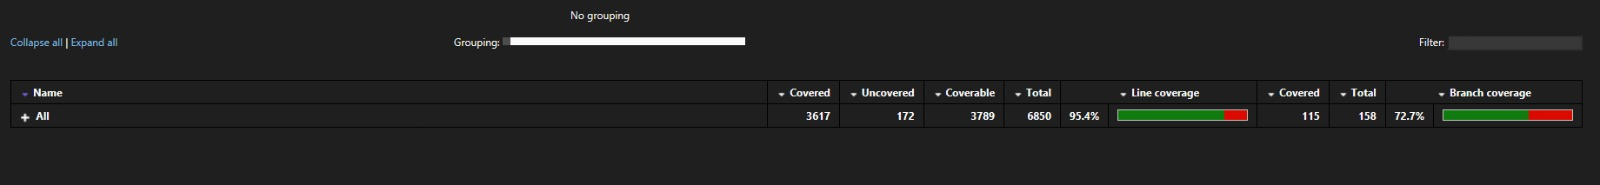
\includegraphics[width=1\textwidth]{imagens/testes/TestesUnitariosBackend/coverageGeral.jpeg}
    \label{coverageGeralBack}
	\fonte{Os autores}
\end{figure}

\begin{figure}[H]
    \caption{Cobertura dos testes por camada}
	\centering
	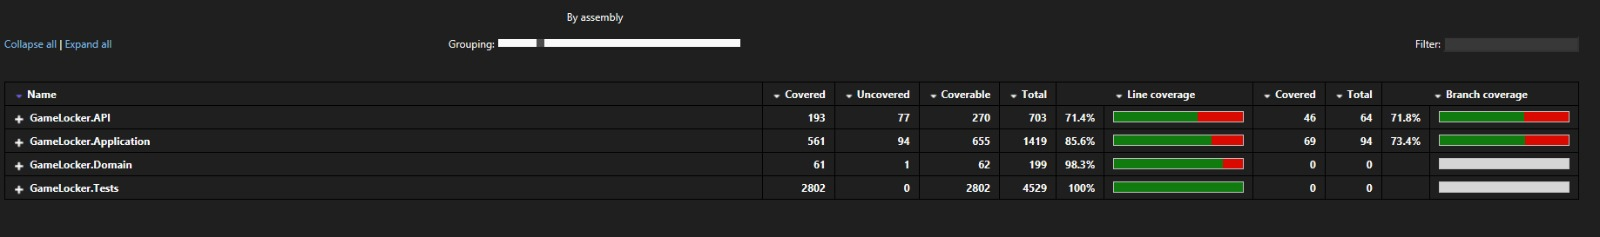
\includegraphics[width=1\textwidth]{imagens/testes/TestesUnitariosBackend/coverage.jpeg}
	\label{coverageBack}
    \fonte{Os autores}
\end{figure}
\pagebreak

A figura \ref{resultadoTestesBack} apresenta o resultado da execução dos testes, demonstrando sucesso em todos eles.

\begin{figure}[H]
    \caption{Resultado dos testes}
	\centering
	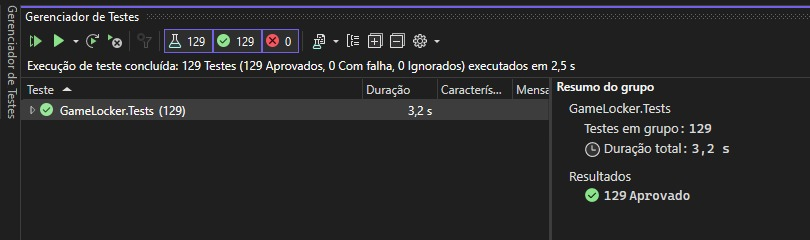
\includegraphics[width=1\textwidth]{imagens/testes/TestesUnitariosBackend/resultado.jpeg}
    \label{resultadoTestesBack}
	\fonte{Os autores}
\end{figure}

\subsection{Front-end}
Para auxiliar no desenvolvimento dos testes unitários do \textit{\gls{Front-end}}, foram utilizadas as bibliotecas \textit{Jest} e \textit{React Testing Library}.

A figura \ref{coverageFront} demonstra a cobertura de testes por página da aplicação. Já a figura \ref{coverageGeralFront} apresenta a cobertura geral, em todos os arquivos.

\begin{figure}[H]
    \caption{Cobertura dos testes por página}
	\centering
	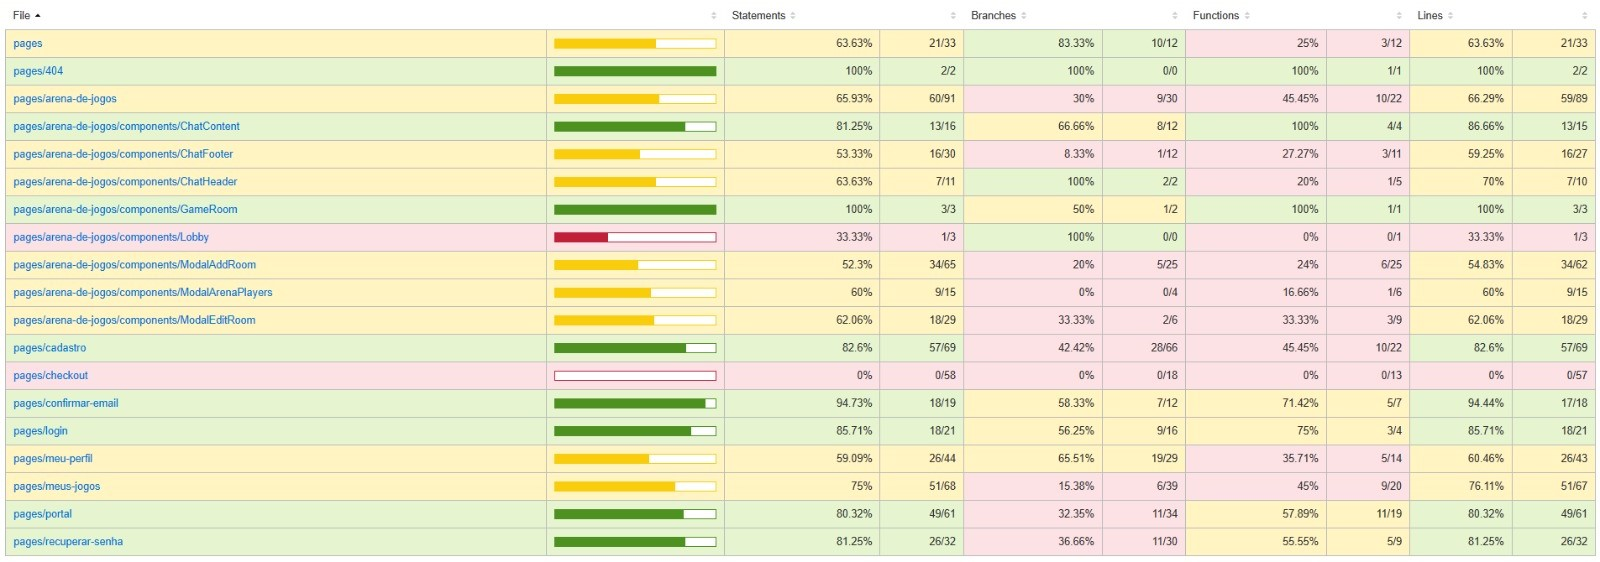
\includegraphics[width=1\textwidth]{imagens/testes/TestesUnitariosFrontend/coverageFront.jpeg}
	\label{coverageFront}
    \fonte{Os autores}
\end{figure}

\begin{figure}[H]
    \caption{Cobertura Geral dos testes}
	\centering
	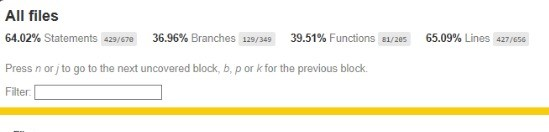
\includegraphics[width=1\textwidth]{imagens/testes/TestesUnitariosFrontend/coverageGeralFront.jpeg}
	\label{coverageGeralFront}
    \fonte{Os autores}
\end{figure}

Na figura \ref{resultadosTestesFront} é possível observar o resultado da execução dos testes, demonstrando êxito em sua totalidade.

\begin{figure}[H]
    \caption{Resultados dos testes}
	\centering
	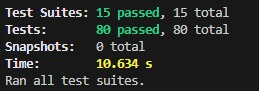
\includegraphics[width=1\textwidth]{imagens/testes/TestesUnitariosFrontend/resultadosTestesFront.jpeg}
	\label{resultadosTestesFront}
    \fonte{Os autores}
\end{figure}